\documentclass[11pt]{amsart}
\usepackage[margin=1in]{geometry}                % See geometry.pdf to learn the layout options. There are lots.
\geometry{letterpaper}                   % ... or a4paper or a5paper or ... 
%\geometry{landscape}                % Activate for for rotated page geometry
%\usepackage[parfill]{parskip}    % Activate to begin paragraphs with an empty line rather than an indent
\usepackage{graphicx}
\usepackage{amssymb}
\usepackage{epstopdf}
\DeclareGraphicsRule{.tif}{png}{.png}{`convert #1 `dirname #1`/`basename #1 .tif`.png}

\title{Math 228b, Spring 2014, homework 1}
\author{Jake Edman}
\date{}                                           % Activate to display a given date or no date

\begin{document}
\maketitle
\section{solve $u_t = u_{xx}$ on [0,1] with I.C. $u(x,0)= \sin(\pi x)$}
\subsection{$h=k=1/10$}
Figure \ref{u1} depicts the solution at $t=1$.  This solution is clearly very bad, and unstable. Heat should diffuse out along the domain, away from the initial maximum at $x=0.5$, and because there are no sources or sinks in the domain, it should simply flatten out to zero over time, and never become negative.  Additionally, the solution should be symmetrical along the x axis; the initial condition and boundary conditions are symmetric, and there are no sources or sinks to break the symmetry. The solution depicted in figure \ref{u1} changes sign as we move along the x axis, and is not symmetric, which must arise from  numerical instability. Instability is expected; in class, we showed that this scheme is stable for $\lambda \equiv \frac{k}{h^2} \le \frac{1}{2}$, and in this case $\lambda = 10$. 

\begin{figure}[t]
\begin{center} 
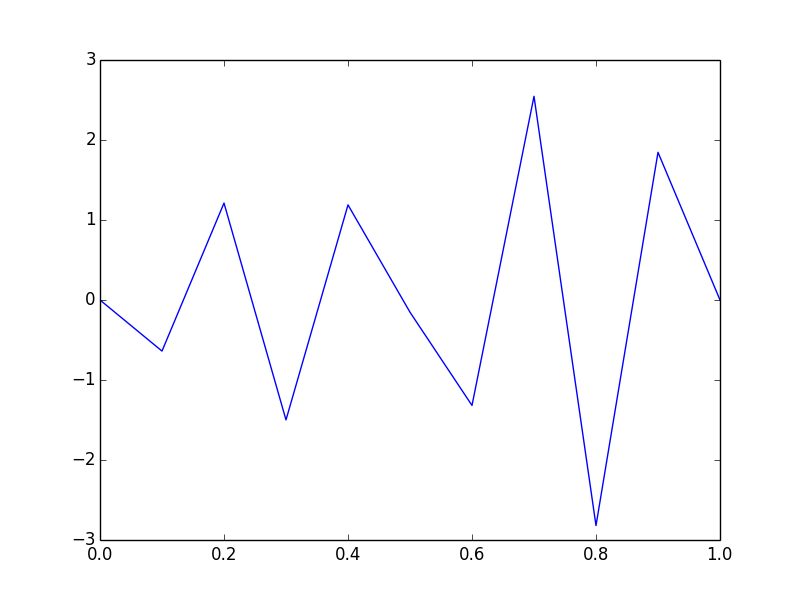
\includegraphics[width=5in,angle=0]{u1.pdf}
\caption{The solution to $u_t = u_{xx}$ with  $h=k=1/10$ }
\label{u1} 
\end{center}
\end{figure}
  
\subsection{$h=1/10$, $k=1/200$}
The solid blue line in figure \ref{u2} depicts the solution at $t=1$. Unlike the solution depicted in figure \ref{u1}, this solution appears stable, because it is smooth, nonnegative, and symmetric. We expect stability, because $\lambda = 1/2$ in this case. 

\begin{figure}[t]
\begin{center} 
\includegraphics[width=5in,angle=0]{u1_2_conv.pdf}
\caption{The solution to $u_t = u_{xx}$ with $\lambda = 1/2$ for a range of meshes.}
\label{u2} 
\end{center}
\end{figure}

\subsection{$\lambda = 1/6$} 

\begin{figure}[t]
\begin{center} 
\includegraphics[width=5in,angle=0]{u1_6_conv.pdf}
\caption{The solution to $u_t = u_{xx}$ with  $\lambda =1/6$ for a range of meshes.  }
\label{u16} 
\end{center}
\end{figure}

The dashed green line in figure \ref{u2} depicts the solution at $t=1$ for $\lambda =1/6$. This solution is clearly different than the one given by $\lambda =1/2$, but is it `better'? 

In class, we showed that truncation error is minimized for $\lambda = 1/6$;  the truncation error is defined as $\tau^k_h = u^{k}_h - u_{exact}$ where the superscript $u_h^k$ refer to the solution on a grid defined by space and  time discretization $h$ and $k$, respectively , and $u^{exact}$ is the exact solution. Assuming the truncation error can be related to the discretization raised to some exponent $a$, such that $\tau_h = Ch^a$, where $C$ is a constant and $a$ is the order of convergence in space, we can write  
\begin{eqnarray} 
Ch_1^a = u_{h_1} - u_{exact}\\
Ch_2^a= u_{h_2} - u_{exact}\\
Ch_3^a = u_{h_3} - u_{exact}
\end{eqnarray} 
To compare the convergence rate for different $k$, we need to approximate $u_{exact}$ somehow. We can solve this system for $a$ and approximate $u_{exact}$ if we choose grids such that $k_3/k_2 = k_2/k_1 =$ constant. Eliminating $u_{exact}$ and taking $h_2/h_1 = h_3/h_2 = r$ , the system becomes
\begin{eqnarray} 
\frac{u_{h_3}-u_{h_2}}{u_{h_2}-u_{h_1}} &=& \left(\frac{h_2}{h_1}\right)^a \left[\frac{(h_3/h_2)^a -1}{(h_2/h_1)^a-1}\right]\\
\ln\left( \frac{u_{h_3}-u_{h_2}}{u_{h_2}-u_{h_1}}\right) &=&  a \ln \left(r\right)
\end{eqnarray} 

From this expression, we can compute the order of convergence $a$ in space from an experiment where we refine the mesh by a constant ratio $r$. By substituting $k$'s for $h$'s in the above derivation, we could also compute the order of convergence in time.  

To compare the order of convergence for $\lambda = 1/6$ and $\lambda = 1/2$, we can run two sets of  three simulations, where we double the spatial refinement twice but keep $ \lambda$ fixed. 
For this set of experiments, I chose to halve the spatial discretization each time (e.g. $h_2/h_1$ = 2), so for fixed $\lambda$,  $r =k_2/k_1$ =4. Both of these values are computed in the script convergence.py, where we find that for $\lambda = 1/6$, the error is order 4 in space and order 2 in time. On the other hand, for $\lambda =1/2$,   the error is order 2 in space and  but still order 2 in time. This improved convergence can be readily seen by comparing figures \ref{u2} and \ref{u16}, as the solutions with $\lambda =1/6$ are nearly identical for all spatial discretizations, but have not yet converged for $\lambda = 1/2$.

\section{Comparison with exact solution for  I.C. $u(x,0)= \sin(\pi x)$} 

\section{Comparison with exact solution for  I.C. $u(x,0)= x(1-x)$} 

\section{Consider $u_t = \alpha u_{xx}$ on [0,1] with I.C. $u(x,0)= \sin(\pi x)$, where $\alpha$ is a constant. }


\section{Consider $u_t = \alpha(x) u_{xx}$ on [0,1] with I.C. $u(x,0)= \sin(\pi x)$ }


\end{document}  